% -------------- Some basic Tikz

\documentclass[10pt,a4paper,twoside]{article}
\usepackage[utf8]{inputenc}
\usepackage{amsmath}
\usepackage{amsfonts}
\usepackage{amssymb}
\usepackage{tcolorbox}
\usepackage{pgf,tikz}
\usetikzlibrary{shapes.geometric, arrows}
\usetikzlibrary{automata, positioning, arrows}
\usepackage{multicol}
\usepackage{hyperref} %required for table of contents
\usepackage{graphicx}
\usepackage[top=1cm,left=1cm,width = 14cm]{geometry}
\author{}
\title{\textbf{Subject: Basic Lines on Graphs}}

% new tcolorbox environment
% #1: tcolorbox options
% #2: color
% #3: box title
\newtcolorbox{mybox}[3][]
{
  colframe = #2!25, colback  = #2!10, coltitle = #2!20!black, title    = {#3}, #1,
}

% -------------------------------------------------------------------------------------------
\begin{document}
\maketitle{}
\marginparwidth=4.5cm
\begin{mybox}{blue}{Objectives}
\begin{itemize}
\item A few simple diagrams for plotting graphs
\end{itemize}
\end{mybox}

To include a graph you can use the following code
\begin{verbatim}

\begin{tikzpicture}
	\draw[step=1cm,gray,very thin] (0,0) grid (4,4);
\end{tikzpicture}\\
\end{verbatim}
which produces:


\begin{tikzpicture}
	\draw[step=1cm,gray,very thin] (0,0) grid (4,4);
\end{tikzpicture}\\

To overlay lines, do this
\begin{verbatim}
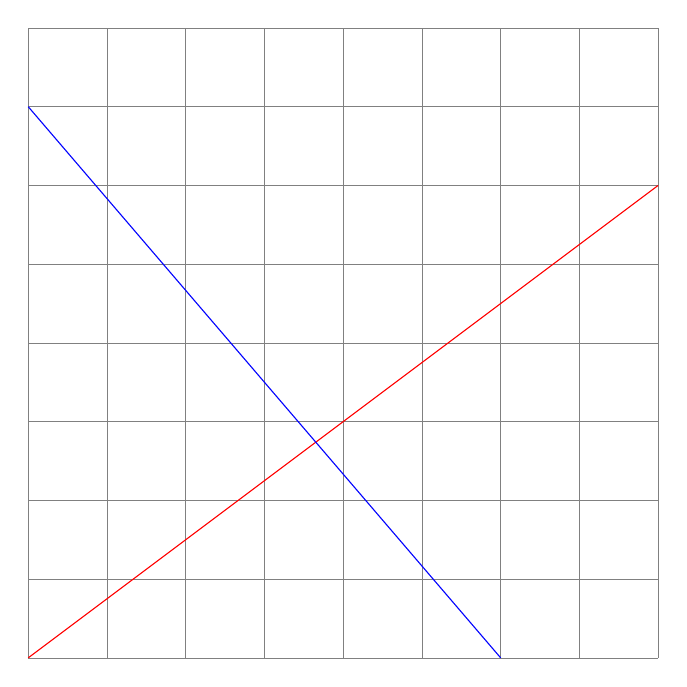
\begin{tikzpicture}
	\draw[step=1cm,gray,very thin] (0,0) grid (8,8);
	\draw [red] (0,0) -- (8,6);
	\draw [blue] (0,7) -- (6,0);
\end{tikzpicture}\\
\end{verbatim}

which produces

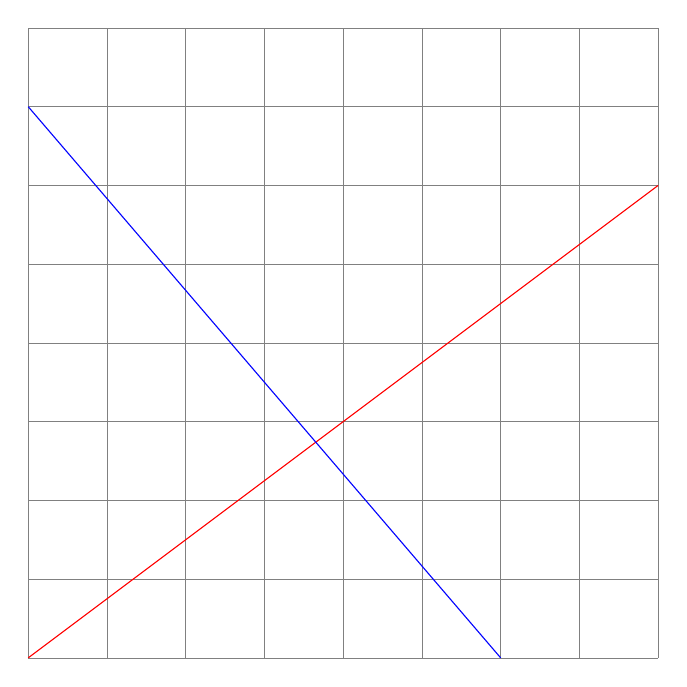
\begin{tikzpicture}
	\draw[step=1cm,gray,very thin] (0,0) grid (8,8);
	\draw [red] (0,0) -- (8,6);
	\draw [blue] (0,7) -- (6,0);
\end{tikzpicture}\\

If you want to include axis:

\begin{verbatim}
 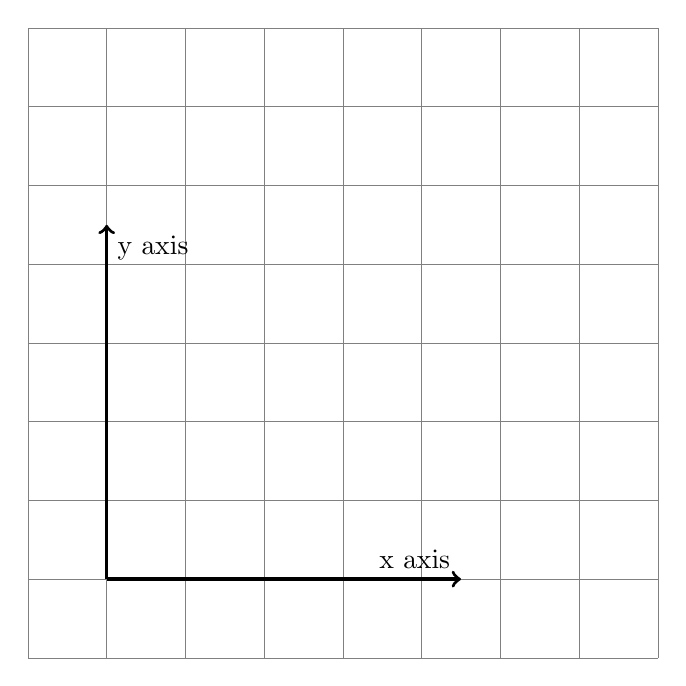
\begin{tikzpicture}
	\draw[step=1cm,gray,very thin] (-1,-1) grid (7,7);
	\draw[very thick,->] (0,0) -- (4.5,0)node[anchor=south east] {x axis};
	\draw[very thick,->] (0,0) -- (0,4.5) 		node[anchor=north west] {y axis};
\end{tikzpicture}
\caption{A graph}
\end{verbatim}

 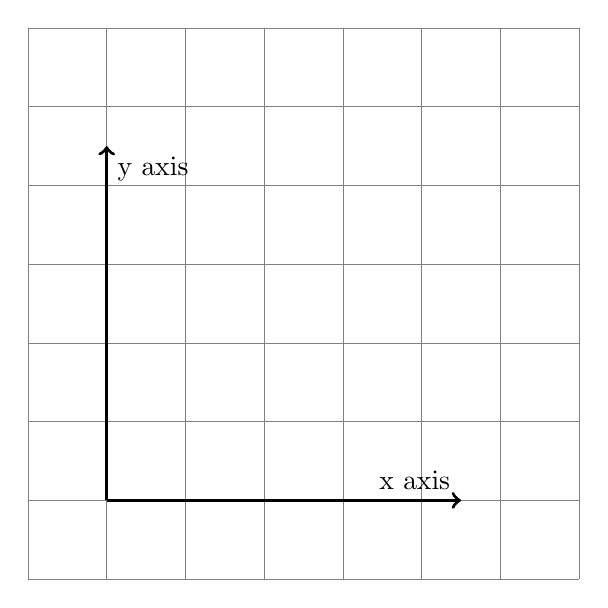
\begin{tikzpicture}
	\draw[step=1cm,gray,very thin] (-1,-1) grid (6,6);
	\draw[very thick,->] (0,0) -- (4.5,0)node[anchor=south east] {x axis};
	\draw[very thick,->] (0,0) -- (0,4.5) 		node[anchor=north west] {y axis};
\end{tikzpicture}

And here is a rectangle:

\begin{verbatim}
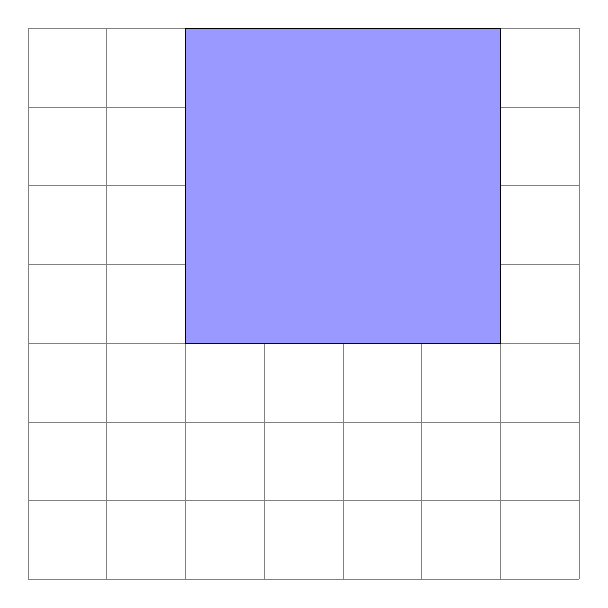
\begin{tikzpicture}
	\draw[step=1cm,gray,very thin] (0,0) grid (7,7);
	\fill[blue!40!white, draw=black] (2,3) rectangle (6,7);
\end{tikzpicture}\\
\end{verbatim}

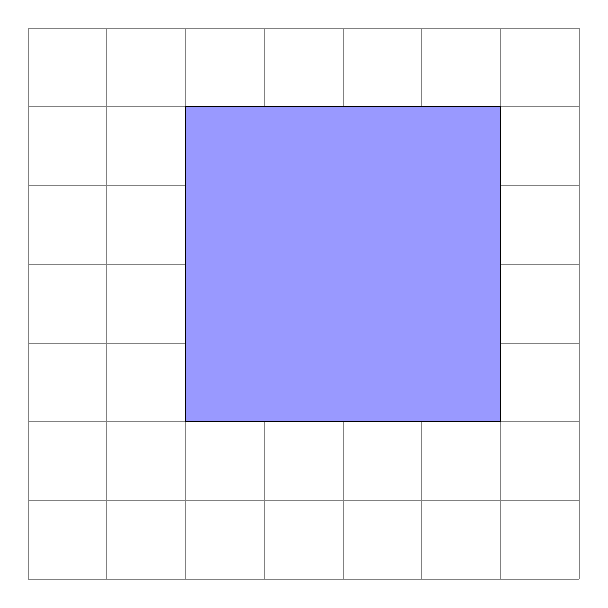
\begin{tikzpicture}
	\draw[step=1cm,gray,very thin] (0,0) grid (7,7);
	\fill[blue!40!white, draw=black] (2,2) rectangle (6,6);
\end{tikzpicture}\\





\end{document}

